\documentclass[11pt]{article}

\usepackage[margin=1in]{geometry}
\usepackage{amsmath,amssymb}
\usepackage{booktabs}
\usepackage{graphicx}
\usepackage{hyperref}
\usepackage{xcolor}
\usepackage{tikz}
\usetikzlibrary{arrows.meta,positioning,shapes.geometric}

\title{Trade Offs between TRM/LDT Hybrids}
\author{Hybrid LDT/TRM Research Gym}
\date{\today}

\newcommand{\envsound}{\textsc{environment-sound}}
\newcommand{\modelsound}{\textsc{model-sound}}
\newcommand{\expsound}{\textsc{experience-sound}}

\begin{document}
\maketitle

\begin{abstract}
We study a small hybrid reasoning architecture that combines a Tiny Recursive Model (TRM) style proposal mechanism with an explicit Lattice Deduction Transformer (LDT) style state. The central design is a typed membrane: the latent side proposes refinements, while the explicit lattice side certifies, rejects, or soft-stores them according to provenance. The goal is not to claim that a lattice guarantees correct abstention in all settings. The narrower claim is that an explicit lattice makes abstention, bottom, monotonicity, and provenance inspectable in domains where the relevant mechanics are checkable.

We evaluate this design on five lightweight benchmarks: Sudoku, ARC-1, ARC-2, environment-pointer routing, and a coupled storyworld playing task. Across the saved runs, hybrid matches the best aggregate score in every task family. It improves proposal efficiency in Sudoku and aggregate ARC-2, repairs unsafe TRM actions in storyworld play, and avoids hard-eliminating routes when LDT evidence is only lexical and therefore not environment-sound. The main negative result is that hybrid is not automatically superior: in routing it only ties TRM when LDT candidate sets are treated as soft evidence, and in two ARC-2 instances its heuristic proposal order uses more proposals than raw TRM.

We also specify a Conductor-HRM review layer for newly trained models. It combines target-blind spectral bundles, checkpoint lineage, loop holonomy, and a conservative signed-control bound with separate held-out utility, damage, provenance, and resource gates. A deterministic receipt-contract exercise validates authorize, section, audit, and reject control flow; it is not reported as neural model-training performance.
\end{abstract}

\section{Motivation}

The motivating question is practical:
\begin{quote}
Can persistent latent recurrence improve explicit lattice deduction without destroying the interpretability and soundness benefits of an explicit abstract state?
\end{quote}

We separate two roles. TRM is private recurrent or heuristic workspace that proposes actions, refinements, routes, or candidate rules. LDT is explicit public lattice state that supports monotone refinement, bottom detection, serialization, and typed provenance. The hybrid architecture is useful only if these roles remain separated. If latent proposals can directly mutate durable state, the system loses the main benefit of explicit deduction. If the lattice is the only mechanism, the system struggles when local propagation is insufficient and search or heuristic proposal is needed.

The terminology is motivated by recent compact recurrent reasoners, especially HRM and TRM~\cite{wang2025hrm,jolicoeurmartineau2025trm}, and by LDT's explicit lattice-state view~\cite{davis2026ldt}. The control-flow question is also adjacent to neurosymbolic architecture taxonomies and systems that combine neural proposal with symbolic, logical, or executable structure~\cite{kautz2022third,garcez2020neurosymbolic,manhaeve2018deepproblog,dong2019nlm,yao2022react}. Our contribution is narrower than that literature: we study when a typed membrane should convert a proposal into a durable lattice update, keep it as soft telemetry, or reject it.

This paper intentionally excludes VPD. The benchmark argument is about hybrid reasoning behavior, typed state updates, and empirical task performance.

\section{Architecture}

At step $t$, the hybrid keeps two states:
\[
  a_t \quad \text{explicit abstract state}, \qquad
  h_t \quad \text{private latent or heuristic state}.
\]

The public state $a_t$ is serializable and checkable. In the implementation, it is often a candidate-set lattice, but the same interface covers intervals, symbolic constraints, reachable regions, possible rules, and possible environment IDs. The private state $h_t$ ranks proposals and tracks search context. It does not directly mutate $a_t$.

\begin{figure}[t]
\centering
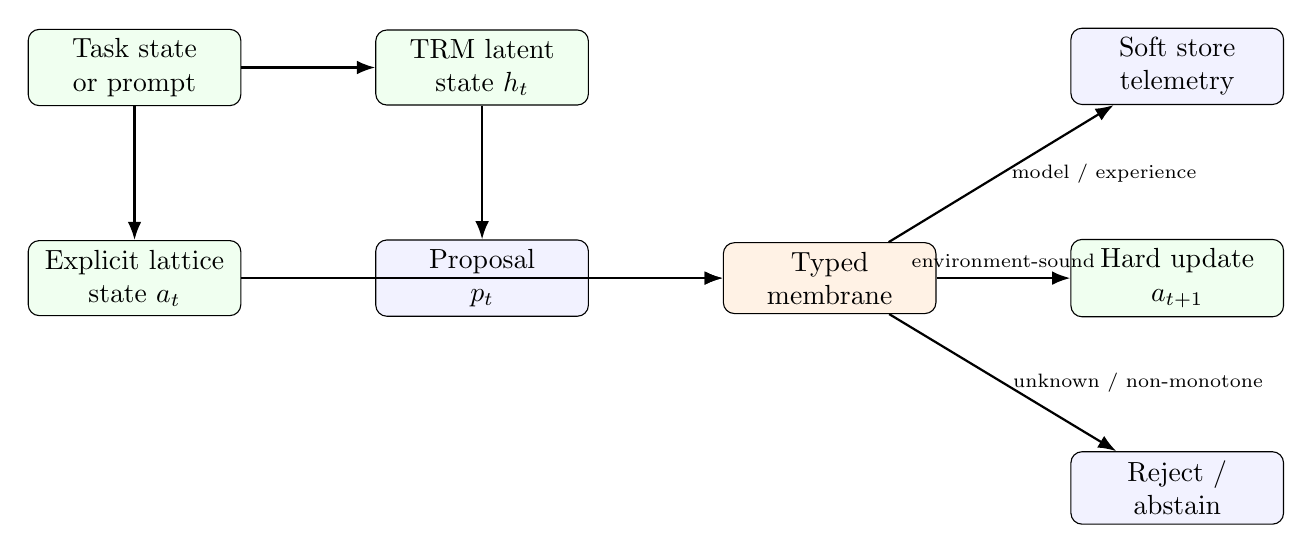
\begin{tikzpicture}[
  node distance=1.7cm and 1.7cm,
  block/.style={draw, rounded corners, align=center, minimum width=2.7cm, minimum height=0.9cm, fill=blue!5},
  state/.style={draw, rounded corners, align=center, minimum width=2.7cm, minimum height=0.9cm, fill=green!6},
  warn/.style={draw, rounded corners, align=center, minimum width=2.7cm, minimum height=0.9cm, fill=orange!10},
  arrow/.style={-Latex, thick}
]
\node[state] (task) {Task state\\or prompt};
\node[state, right=of task] (latent) {TRM latent\\state $h_t$};
\node[state, below=of task] (lattice) {Explicit lattice\\state $a_t$};
\node[block, right=of lattice] (proposal) {Proposal\\$p_t$};
\node[warn, right=of proposal] (membrane) {Typed\\membrane};
\node[state, right=of membrane] (hard) {Hard update\\$a_{t+1}$};
\node[block, above=of hard] (soft) {Soft store\\telemetry};
\node[block, below=of hard] (reject) {Reject /\\abstain};

\draw[arrow] (task) -- (latent);
\draw[arrow] (task) -- (lattice);
\draw[arrow] (latent) -- (proposal);
\draw[arrow] (lattice) -- (membrane);
\draw[arrow] (proposal) -- (membrane);
\draw[arrow] (membrane) -- node[above, font=\scriptsize]{environment-sound} (hard);
\draw[arrow] (membrane) -- node[right, font=\scriptsize]{model / experience} (soft);
\draw[arrow] (membrane) -- node[right, font=\scriptsize]{unknown / non-monotone} (reject);
\end{tikzpicture}

\caption{Hybrid LDT/TRM control loop. The TRM side proposes; the membrane decides whether the proposal can become a durable lattice update.}
\label{fig:architecture}
\end{figure}

\section{Lattice Formulation}

For the candidate-state implementation, following the lattice view used in abstract interpretation~\cite{cousot1977abstract}, let slots be indexed by $i \in I$. Each slot has finite universe $U_i$. A lattice state is
\[
  a = \{ C_i \subseteq U_i \}_{i \in I}.
\]
The top state is
\[
  \top = \{ U_i \}_{i \in I},
\]
and bottom is
\[
  \bot(a) \iff \exists i \in I : C_i = \emptyset.
\]

Meet is pointwise intersection:
\[
  (a \wedge b)_i = C_i^a \cap C_i^b.
\]

A proposal $p_t$ contains a proposed state $\hat a_{t+1}$. It is monotone only if
\[
  \forall i \in I,\quad \hat C_{i,t+1} \subseteq C_{i,t}.
\]
The implementation rejects non-monotone proposals before applying meet:
\[
  \operatorname{reject}(p_t) \quad \text{if} \quad \exists i:\hat C_{i,t+1} \nsubseteq C_{i,t}.
\]
This matters because otherwise a widening proposal could be hidden by a subsequent meet and appear harmless.

\section{Typed Soundness and the Membrane}

Each proposal carries provenance:
\begin{itemize}
  \item \envsound: derived from trusted environment mechanics.
  \item \modelsound: derived from a model of another agent or learned predictor.
  \item \expsound: derived from replay or discovered successes.
  \item unknown: no usable provenance.
\end{itemize}

The default membrane policy is:
\[
\operatorname{hard}(p)=
\begin{cases}
1 & \text{if provenance}(p)=\envsound,\\
0 & \text{otherwise.}
\end{cases}
\]

The durable transition is
\[
a_{t+1} =
\begin{cases}
a_t \wedge \hat a_{t+1} &
\text{if } \operatorname{hard}(p_t)\land \hat a_{t+1}\sqsubseteq a_t
\land \neg\bot(a_t\wedge\hat a_{t+1}),\\
a_t & \text{otherwise.}
\end{cases}
\]

Bottom is allowed only in explicit abstain or conflict mode:
\[
  \bot(a_t \wedge \hat a_{t+1}) \Rightarrow
  \text{accept only if mode}=\textsc{abstain}.
\]

\begin{figure}[t]
\centering
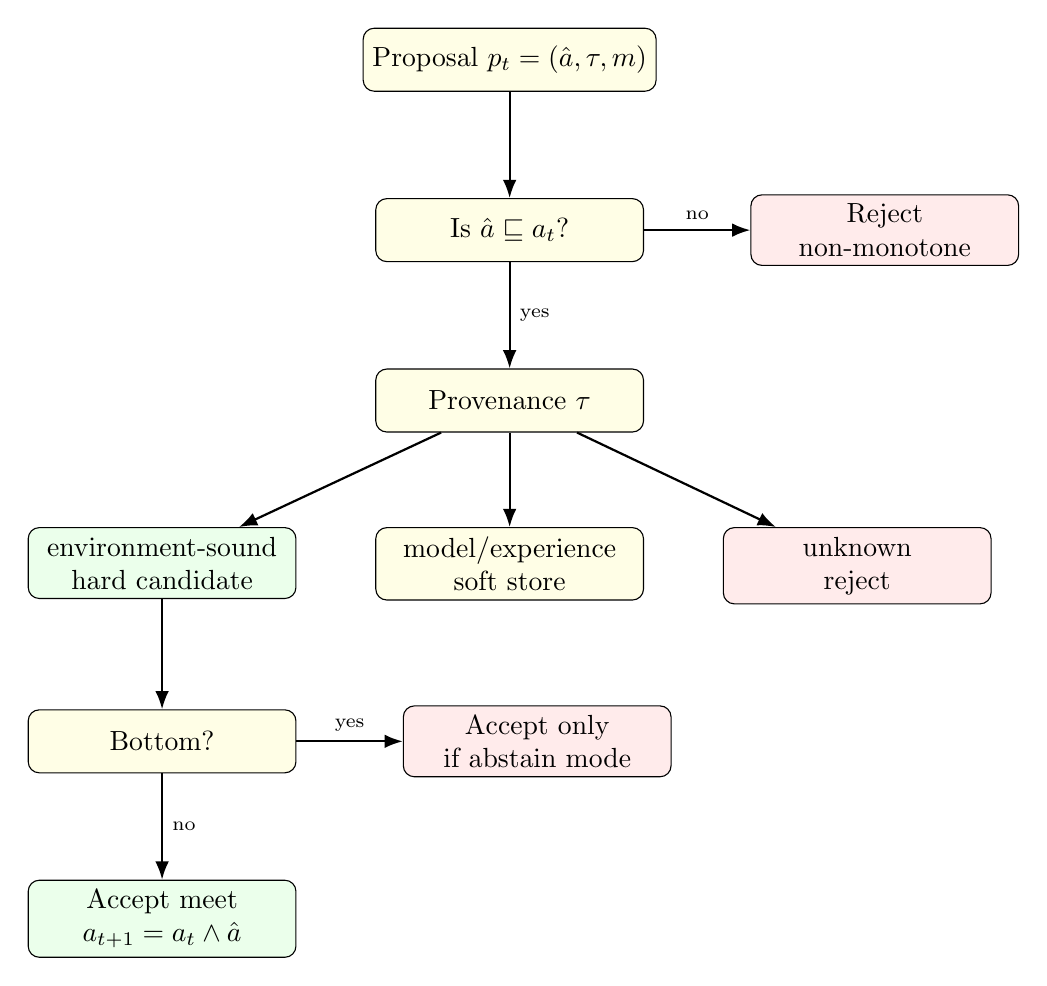
\begin{tikzpicture}[
  node distance=1.35cm,
  box/.style={draw, rounded corners, align=center, minimum width=3.4cm, minimum height=0.8cm},
  yes/.style={box, fill=green!8},
  no/.style={box, fill=red!8},
  mid/.style={box, fill=yellow!10},
  arrow/.style={-Latex, thick}
]
\node[mid] (p) {Proposal $p_t=(\hat a, \tau, m)$};
\node[mid, below=of p] (mono) {Is $\hat a \sqsubseteq a_t$?};
\node[no, right=of mono] (reject1) {Reject\\non-monotone};
\node[mid, below=of mono] (prov) {Provenance $\tau$};
\node[yes, below left=1.2cm and 1.0cm of prov] (env) {environment-sound\\hard candidate};
\node[mid, below=1.2cm of prov] (soft) {model/experience\\soft store};
\node[no, below right=1.2cm and 1.0cm of prov] (unk) {unknown\\reject};
\node[mid, below=1.4cm of env] (bottom) {Bottom?};
\node[yes, below=of bottom] (apply) {Accept meet\\$a_{t+1}=a_t\wedge\hat a$};
\node[no, right=of bottom] (abstain) {Accept only\\if abstain mode};

\draw[arrow] (p) -- (mono);
\draw[arrow] (mono) -- node[above, font=\scriptsize]{no} (reject1);
\draw[arrow] (mono) -- node[right, font=\scriptsize]{yes} (prov);
\draw[arrow] (prov) -- (env);
\draw[arrow] (prov) -- (soft);
\draw[arrow] (prov) -- (unk);
\draw[arrow] (env) -- (bottom);
\draw[arrow] (bottom) -- node[right, font=\scriptsize]{no} (apply);
\draw[arrow] (bottom) -- node[above, font=\scriptsize]{yes} (abstain);
\end{tikzpicture}

\caption{Default membrane policy. Only environment-sound monotone refinements become hard updates. Model-sound and experience-sound proposals can be retained as soft telemetry.}
\label{fig:membrane}
\end{figure}

\section{Control Dynamics and Alternative Architectures}

The typed membrane is one point in a larger design space. We compare it with two implementable alternatives in order to separate the value of hybridization from the risks introduced by the control policy.

\begin{figure}[t]
\centering
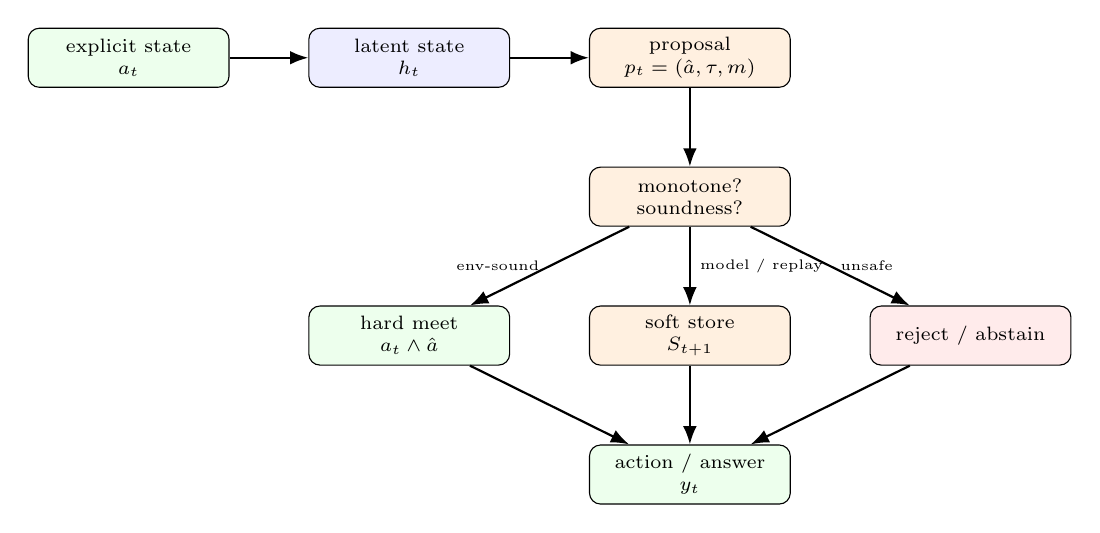
\begin{tikzpicture}[
  node distance=1.0cm and 1.0cm,
  box/.style={draw, rounded corners, align=center, minimum width=2.55cm, minimum height=0.75cm, font=\scriptsize},
  state/.style={box, fill=green!7},
  latent/.style={box, fill=blue!7},
  gate/.style={box, fill=orange!12},
  stop/.style={box, fill=red!8},
  arrow/.style={-Latex, thick}
]
\node[state] (a) {explicit state\\$a_t$};
\node[latent, right=of a] (h) {latent state\\$h_t$};
\node[gate, right=of h] (p) {proposal\\$p_t=(\hat a,\tau,m)$};
\node[gate, below=of p] (check) {monotone?\\soundness?};
\node[state, below left=of check] (hard) {hard meet\\$a_t \wedge \hat a$};
\node[gate, below=of check] (soft) {soft store\\$S_{t+1}$};
\node[stop, below right=of check] (reject) {reject / abstain};
\node[state, below=of soft] (act) {action / answer\\$y_t$};

\draw[arrow] (a) -- (h);
\draw[arrow] (h) -- (p);
\draw[arrow] (p) -- (check);
\draw[arrow] (check) -- node[left, font=\tiny]{env-sound} (hard);
\draw[arrow] (check) -- node[right, font=\tiny]{model / replay} (soft);
\draw[arrow] (check) -- node[right, font=\tiny]{unsafe} (reject);
\draw[arrow] (hard) -- (act);
\draw[arrow] (soft) -- (act);
\draw[arrow] (reject) -- (act);
\end{tikzpicture}

\caption{Control dynamic for the typed membrane. TRM proposes; the membrane decides whether the proposal becomes a hard meet, soft telemetry, or a rejection.}
\label{fig:control-dynamics}
\end{figure}

Let $q_\theta$ denote the TRM proposal or scoring mechanism. In the typed membrane,
\[
  p_t = q_\theta(h_t,a_t,x_t), \qquad
  p_t = (\hat a_{t+1},\tau_t,m_t),
\]
and durable state changes only through the membrane:
\[
a_{t+1} =
\begin{cases}
a_t \wedge \hat a_{t+1} & \tau_t=\envsound,\ \hat a_{t+1}\sqsubseteq a_t,\ \neg\bot(a_t\wedge\hat a_{t+1}),\\
a_t & \text{otherwise.}
\end{cases}
\]

The first alternative is a hard-gated cascade. The LDT state is treated as a mandatory candidate filter:
\[
  C_t = \operatorname{LDT}(x_t), \qquad
  y_t = \arg\max_{y\in C_t} q_\theta(y\mid x_t).
\]
This is attractive when $C_t$ is environment-sound, but unsafe when $C_t$ is lexical or learned. The routing ablation below is exactly this failure mode.

The second alternative is confidence arbitration. Let $s_1(x_t)$ and $s_2(x_t)$ be the top two TRM scores and let
\[
  \Delta_t=s_1(x_t)-s_2(x_t).
\]
Then
\[
y_t =
\begin{cases}
\arg\max_y q_\theta(y\mid x_t) & \Delta_t\ge\gamma,\\
\arg\max_{y\in C_t} q_\theta(y\mid x_t) & \Delta_t<\gamma.
\end{cases}
\]
The threshold $\gamma$ is selected on the training split from a small deterministic grid. On the saved routing run the selected value is $\gamma=0$, meaning that any positive use of noisy LDT routing candidates reduces training accuracy; the arbitration architecture therefore degenerates to TRM on this slice.

\begin{figure}[t]
\centering
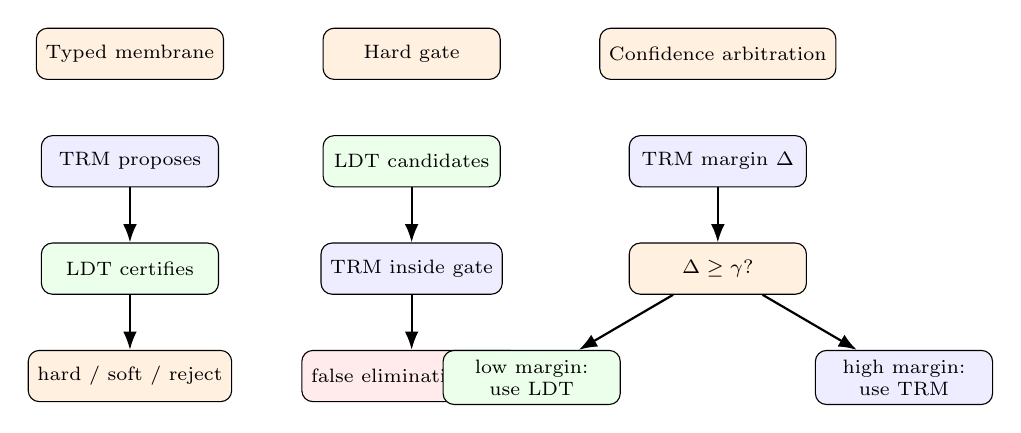
\begin{tikzpicture}[
  node distance=0.7cm and 0.55cm,
  box/.style={draw, rounded corners, align=center, minimum width=2.25cm, minimum height=0.65cm, font=\scriptsize},
  ldt/.style={box, fill=green!8},
  trm/.style={box, fill=blue!7},
  hyb/.style={box, fill=orange!12},
  warn/.style={box, fill=red!8},
  arrow/.style={-Latex, thick}
]
\node[hyb] (tm-title) {Typed membrane};
\node[trm, below=of tm-title] (tm-trm) {TRM proposes};
\node[ldt, below=of tm-trm] (tm-ldt) {LDT certifies};
\node[hyb, below=of tm-ldt] (tm-out) {hard / soft / reject};
\draw[arrow] (tm-trm) -- (tm-ldt);
\draw[arrow] (tm-ldt) -- (tm-out);

\node[hyb, right=1.25cm of tm-title] (hg-title) {Hard gate};
\node[ldt, below=of hg-title] (hg-ldt) {LDT candidates};
\node[trm, below=of hg-ldt] (hg-trm) {TRM inside gate};
\node[warn, below=of hg-trm] (hg-out) {false elimination risk};
\draw[arrow] (hg-ldt) -- (hg-trm);
\draw[arrow] (hg-trm) -- (hg-out);

\node[hyb, right=1.25cm of hg-title] (ca-title) {Confidence arbitration};
\node[trm, below=of ca-title] (ca-trm) {TRM margin $\Delta$};
\node[hyb, below=of ca-trm] (ca-switch) {$\Delta \ge \gamma$?};
\node[ldt, below left=0.7cm and 0.1cm of ca-switch] (ca-ldt) {low margin:\\use LDT};
\node[trm, below right=0.7cm and 0.1cm of ca-switch] (ca-direct) {high margin:\\use TRM};
\draw[arrow] (ca-trm) -- (ca-switch);
\draw[arrow] (ca-switch) -- (ca-ldt);
\draw[arrow] (ca-switch) -- (ca-direct);
\end{tikzpicture}

\caption{Three benchmarked hybrid control policies: typed membrane, hard-gated cascade, and confidence arbitration.}
\label{fig:architecture-comparison}
\end{figure}

\section{Practical Hybrid Dynamics}

The hybrid does not play the same role in every domain. Figure~\ref{fig:patterns} summarizes the main patterns.

\begin{figure}[t]
\centering
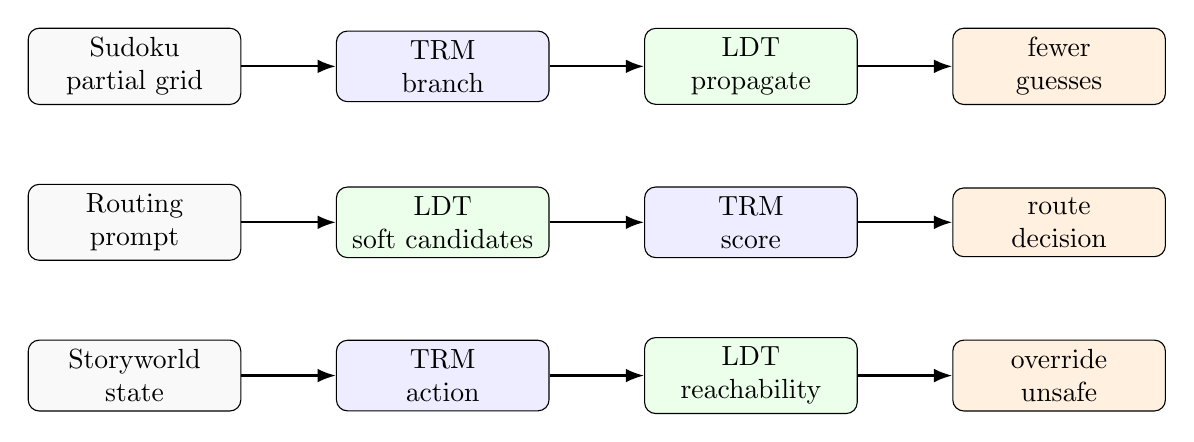
\begin{tikzpicture}[
  node distance=1.0cm and 1.2cm,
  box/.style={draw, rounded corners, align=center, minimum width=2.7cm, minimum height=0.85cm, fill=gray!5},
  ldt/.style={box, fill=green!8},
  trm/.style={box, fill=blue!7},
  hyb/.style={box, fill=orange!12},
  arrow/.style={-Latex, thick}
]
\node[box] (sudoku) {Sudoku\\partial grid};
\node[trm, right=of sudoku] (branch) {TRM\\branch};
\node[ldt, right=of branch] (prop) {LDT\\propagate};
\node[hyb, right=of prop] (solve) {fewer\\guesses};
\draw[arrow] (sudoku) -- (branch);
\draw[arrow] (branch) -- (prop);
\draw[arrow] (prop) -- (solve);

\node[box, below=1.0cm of sudoku] (routing) {Routing\\prompt};
\node[ldt, right=of routing] (cand) {LDT\\soft candidates};
\node[trm, right=of cand] (score) {TRM\\score};
\node[hyb, right=of score] (route) {route\\decision};
\draw[arrow] (routing) -- (cand);
\draw[arrow] (cand) -- (score);
\draw[arrow] (score) -- (route);

\node[box, below=1.0cm of routing] (story) {Storyworld\\state};
\node[trm, right=of story] (act) {TRM\\action};
\node[ldt, right=of act] (reach) {LDT\\reachability};
\node[hyb, right=of reach] (override) {override\\unsafe};
\draw[arrow] (story) -- (act);
\draw[arrow] (act) -- (reach);
\draw[arrow] (reach) -- (override);
\end{tikzpicture}

\caption{Three practical hybrid patterns: branch then propagate, soft route telemetry, and action proposal plus reachability override.}
\label{fig:patterns}
\end{figure}

\subsection{Sudoku}

LDT performs naked-single propagation. TRM performs heuristic minimum-remaining-values search. Hybrid lets TRM propose a branch and then applies LDT propagation after the proposal. TRM is useful for escaping propagation plateaus; LDT is useful immediately after proposals because it collapses implied consequences.

\subsection{ARC-1 and ARC-2}

ARC-1 is a single-rule grid transformation benchmark inspired by the Abstraction and Reasoning Corpus framing~\cite{chollet2019measure}. ARC-2 uses ordered two-rule compositions. LDT derives broad rule-family constraints from input/output invariants. TRM searches primitive rules or ordered pairs. Hybrid restricts proposals by LDT families and certifies them against training examples:
\[
  \operatorname{accept}(\hat r)
  \iff
  \forall (x_j,y_j)\in D_{\text{train}}:\hat r(x_j)=y_j.
\]
For ARC-2, $\hat r = r_b \circ r_a$ and the same certification applies.

\subsection{Environment-Pointer Routing}

Routing maps a prompt to an environment ID. The Tesseract router reference trains a TF-IDF plus MLP router~\cite{tesseract2026router}. The dependency-light benchmark here uses a lexical TRM analogue. LDT builds token-derived candidate sets:
\[
  C_t = \bigcap_{w\in \operatorname{tokens}(x)} E_w,
\]
where $E_w$ is the set of environments associated with token $w$. This evidence is not environment-sound. It is model- or experience-derived. Therefore the final hybrid design uses it as soft guidance only:
\[
\operatorname{route}_{\text{hybrid}}(x)=
\begin{cases}
\arg\max_{e\in C_t}\operatorname{TRM}(e\mid x) &
\text{if TRM top route is in } C_t,\\
\arg\max_e \operatorname{TRM}(e\mid x) & \text{otherwise.}
\end{cases}
\]

\subsection{Storyworld Playing}

The storyworld has exact transitions and a modeled rival policy. LDT uses finite-horizon reachability. TRM uses a greedy local-deficit heuristic. Hybrid lets TRM propose an action, then checks whether the action preserves modeled reachability:
\[
  \operatorname{safe}(s,a,H)
  =
  \operatorname{Reachable}_{\text{model}}(T(s,a,\pi_{\text{rival}}(s)),H-1).
\]
Action selection is:
\[
a_t =
\begin{cases}
a^{\text{TRM}}_t & \text{if safe}(s_t,a^{\text{TRM}}_t,H-t),\\
a^{\text{LDT}}_t & \text{if } a^{\text{LDT}}_t \text{ exists},\\
a^{\text{TRM}}_t & \text{otherwise.}
\end{cases}
\]

This is also where the richer storyworld intuition enters the paper. Secret endings and morality optimization are not the same control problem. A secret ending is a typed gate: the system either preserves reachability to a specific latent ending predicate or it does not. A morality objective is a soft preference surface: it can reward trust, evidence, low heat, and scene progress without being an environment-sound proof obligation. This mirrors the difference between worlds such as medical triage or bioethics councils, where some constraints are hard safety gates while others are soft value tradeoffs.

\section{Results}

\begin{table}[t]
\centering
\begin{tabular}{lrrrr}
\toprule
Benchmark & LDT & TRM & Hybrid & Best \\
\midrule
Sudoku & 0.333 & 1.000 & 1.000 & TRM, Hybrid \\
ARC-1 & 1.000 & 1.000 & 1.000 & All \\
ARC-2 & 1.000 & 1.000 & 1.000 & All \\
Routing & 0.474 & 0.815 & 0.815 & TRM, Hybrid \\
Storyworld & 1.000 & 0.172 & 1.000 & LDT, Hybrid \\
\bottomrule
\end{tabular}
\caption{Saved benchmark scores. Scores are solve rate or routing accuracy depending on the task family.}
\label{tab:results}
\end{table}

The aggregate pattern is:
\begin{itemize}
  \item TRM helps when proposal, search, or lexical classification is needed.
  \item LDT helps when mechanics are explicit and checkable.
  \item Hybrid helps when proposal can be followed by checkable pruning, certification, or reachability checks.
  \item Hybrid does not automatically improve learned routing if the LDT side has only soft lexical evidence.
\end{itemize}

In Sudoku, hybrid matches TRM's solve rate while reducing guesses from 31 to 6. In ARC-1, hybrid matches the best score and uses fewer steps than LDT and fewer proposals than TRM. In ARC-2, hybrid matches the best score and reduces aggregate proposals versus TRM, 32 versus 38, but is inferior to TRM on two individual task proposal counts because the current proposal ordering is heuristic. In routing, hybrid matches TRM accuracy only after treating LDT candidate sets as soft guidance; forcing LDT candidates as hard filters drops accuracy to 0.584. In storyworld play, hybrid matches LDT success and slightly reduces average steps, using 124 overrides to repair unsafe TRM proposals.

\begin{table}[t]
\centering
\begin{tabular}{lrrrr}
\toprule
Routing variant & Accuracy & Correct & Abstained & Avg. candidates \\
\midrule
TRM & 0.815 & 141/173 & 0 & 0.00 \\
Soft hybrid & 0.815 & 141/173 & 0 & 2.09 \\
Hard-filter hybrid & 0.584 & 101/173 & 0 & 2.09 \\
\bottomrule
\end{tabular}
\caption{Routing ablation. Token-lattice candidate sets help as telemetry but are too noisy for hard elimination.}
\label{tab:routing-ablation}
\end{table}

\begin{table}[t]
\centering
\begin{tabular}{lrrl}
\toprule
Architecture & Accuracy & Correct & Control policy \\
\midrule
Typed membrane & 0.815 & 141/173 & soft telemetry unless sound \\
Hard gate & 0.584 & 101/173 & LDT candidates hard-filter TRM \\
Confidence arbitration & 0.815 & 141/173 & train-selected $\gamma=0$ \\
\bottomrule
\end{tabular}
\caption{Implemented routing architecture variants. Hard gating is inferior; confidence arbitration selects the TRM-only boundary on this data.}
\label{tab:architecture-variants}
\end{table}

\begin{table}[t]
\centering
\begin{tabular}{lll}
\toprule
Regime & Preferred policy & Reason \\
\midrule
Environment-sound gate & Typed membrane or hard gate & Proof-like state should dominate confidence \\
Soft preference objective & Confidence arbitration & Local score can optimize value tradeoffs \\
Noisy lexical evidence & Typed membrane & Keep learned candidates soft \\
Checkable search space & Typed membrane & Propose with TRM, certify with LDT \\
\bottomrule
\end{tabular}
\caption{Policy-selection rule of thumb from the saved benchmarks.}
\label{tab:policy-selection}
\end{table}

\begin{table}[t]
\centering
\begin{tabular}{llrr}
\toprule
Scenario & Policy & Success rate & Avg. score \\
\midrule
Secret ending & Typed membrane & 1.000 & 1.00 \\
Secret ending & Confidence arbitration & 0.938 & 0.94 \\
Moral optimization & Typed membrane & 1.000 & 9.95 \\
Moral optimization & Confidence arbitration & 1.000 & 11.06 \\
\bottomrule
\end{tabular}
\caption{Storyworld confidence/type split. Typed reachability wins on hard secret gates; confidence arbitration is useful on a soft morality score.}
\label{tab:storyworld-confidence-type}
\end{table}

\paragraph{Transcript slice.}
One secret-ending run starts at $(\text{trust}=3,\text{evidence}=1,\text{heat}=4,\text{scene}=1)$. Confidence arbitration sees high local margins and repeatedly selects \texttt{defuse}: \texttt{defuse, defuse, defuse, defuse}. It ends at $(3,1,0,5)$ and fails because evidence never reaches the secret gate. The typed membrane instead accepts the need to preserve reachability and follows \texttt{defuse, wait, wait, investigate, defuse, investigate}, ending at $(1,3,2,5)$ and satisfying the secret-ending predicate.

\section{HRM Review of New Model Training}

The multi-module extension uses a Conductor-HRM to schedule review modules rather than directly control model
weights. The slow HRM chooses the review regime and active audit graph. The fast HRM requests spectral,
lineage, holonomy, utility, damage, and resource receipts. A typed join emits one of four routes: authorize,
section into local patches, audit missing evidence, or reject and retain the base model. Figure~\ref{fig:hrm-review}
shows this control flow.

\begin{figure}[t]
\centering
\resizebox{\linewidth}{!}{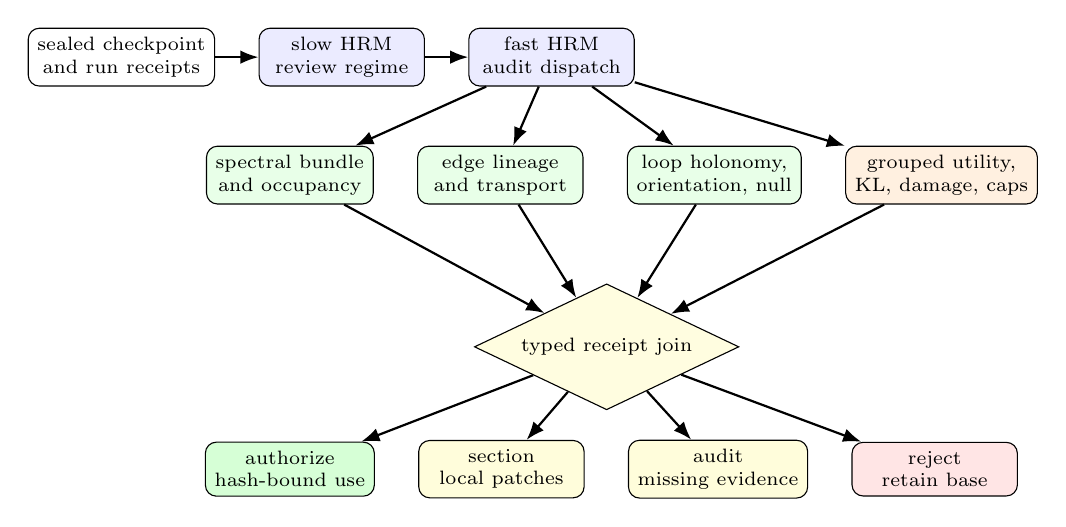
\begin{tikzpicture}[
  node distance=0.62cm and 0.55cm,
  box/.style={draw, rounded corners, align=center, minimum width=2.1cm, minimum height=0.62cm, font=\scriptsize},
  manager/.style={box, fill=blue!8},
  geometry/.style={box, fill=green!9},
  evidence/.style={box, fill=orange!12},
  decision/.style={draw, diamond, aspect=2.1, align=center, fill=yellow!12, font=\scriptsize},
  accept/.style={box, fill=green!16},
  defer/.style={box, fill=yellow!14},
  reject/.style={box, fill=red!10},
  arrow/.style={-Latex, thick}
]
\node[box] (candidate) {sealed checkpoint\\and run receipts};
\node[manager, right=of candidate] (slow) {slow HRM\\review regime};
\node[manager, right=of slow] (fast) {fast HRM\\audit dispatch};

\node[geometry, below left=0.75cm and 1.2cm of fast] (spectral) {spectral bundle\\and occupancy};
\node[geometry, right=of spectral] (lineage) {edge lineage\\and transport};
\node[geometry, right=of lineage] (holonomy) {loop holonomy,\\orientation, null};
\node[evidence, right=of holonomy] (utility) {grouped utility,\\KL, damage, caps};

\node[decision, below=1.0cm of lineage, xshift=1.35cm] (join) {typed receipt join};
\node[accept, below left=0.8cm and 2.1cm of join] (authorize) {authorize\\hash-bound use};
\node[defer, right=of authorize] (section) {section\\local patches};
\node[defer, right=of section] (audit) {audit\\missing evidence};
\node[reject, right=of audit] (reject) {reject\\retain base};

\draw[arrow] (candidate) -- (slow);
\draw[arrow] (slow) -- (fast);
\draw[arrow] (fast) -- (spectral);
\draw[arrow] (fast) -- (lineage);
\draw[arrow] (fast) -- (holonomy);
\draw[arrow] (fast) -- (utility);
\draw[arrow] (spectral) -- (join);
\draw[arrow] (lineage) -- (join);
\draw[arrow] (holonomy) -- (join);
\draw[arrow] (utility) -- (join);
\draw[arrow] (join) -- (authorize);
\draw[arrow] (join) -- (section);
\draw[arrow] (join) -- (audit);
\draw[arrow] (join) -- (reject);
\end{tikzpicture}
}
\caption{RSITopology-aware Conductor-HRM review. Geometry limits the authority of internal-coordinate operations;
behavioral and operational receipts separately control model promotion.}
\label{fig:hrm-review}
\end{figure}

For context stratum $p$, let the normalized reliability-weighted Laplacian be
\[
\widetilde L_p=\frac{\delta_p^\top W_p\delta_p}
{\lambda_{\max}(\delta_p^\top W_p\delta_p)}.
\]
For a frozen spectral interval $I_b$, form $P_b(p)=\mathbf 1_{I_b}(\widetilde L_p)$ and infer a consensus bundle
from projector occupancy:
\[
\overline P_b=\frac{1}{|\mathcal P|}\sum_pP_b(p),\qquad
U_b=\operatorname{im}\mathbf 1_{[\rho,1]}(\overline P_b).
\]
This replaces a guessed rank with an occupancy-derived rank. Cross-site projectors are admitted only after
Jacobians register them into a common edit space. Bundle discovery and all thresholds are sealed before outcome
reveal.

For adjacent orthonormal frames, the overlap decomposes as
\[
U_b^\top U_a=Q_{b\leftarrow a}S_{ba},
\]
where $S_{ba}$ measures principal-angle retention and $Q_{b\leftarrow a}$ transports signed coordinates. Around
a registered context-by-checkpoint loop,
\[
H_{\square}=Q_{00\leftarrow01}Q_{01\leftarrow11}
Q_{11\leftarrow10}Q_{10\leftarrow00},\qquad
\kappa_{\square}=1-\frac{\operatorname{tr}(H_{\square})}{r}.
\]
Good local edge retention does not imply a globally stable signed frame. Loop audits therefore include
orientation and a matched noise null conditioned on rank, perimeter, edge retention, uncertainty, and visibility.

Let $W_e$ be a one-sided lower bound on worst-direction squared retention. For a path with net polar transport
$H$, the signed-coordinate error obeys
\[
\|M-I\|_2\leq\sum_e(1-\sqrt{W_e})+\|H-I\|_2.
\]
For orientation-preserving $H$, $\|H-I\|_2=2\sin(\alpha_{\max}/2)$; orientation reversal or an unmeasured loop
forces the conservative value 2. With simultaneous coverage at least $1-\delta$, global signed control is
authorized only when the uncertainty-adjusted bound $\widehat R\leq\epsilon$. This controls false authorization
for registered signed coordinates. It does not establish behavioral safety.

Invariant bundle energy
\[
e_b(x)=\frac{\|U_b^\top x\|_2^2}{\|x\|_2^2}
\]
needs lineage but not a globally fixed signed basis. It may tilt allocation by
\[
\pi_\eta(i\mid s)\propto\pi_0(i\mid s)\exp(\eta\widehat\Delta_{u,i}),
\qquad D_{\mathrm{KL}}(\pi_\eta\|\pi_0)\leq K_{\max}.
\]
Positive grouped held-out gain, standardized uplift, independent replicates, and matched-rank Haar controls remain
required. Model promotion additionally requires held-out damage, OS-enforced RAM/CPU/I/O caps, chunk and
checkpoint policy, structured resource logs, abort status, process-owned cleanup, and hash-bound provenance.

This yields three identity levels: \texttt{engineering\_evidence}, \texttt{lineage\_certified}, and
\texttt{holonomy\_clean}. Ordinary optimizer promotion needs behavioral and engineering evidence but no signed
coordinate claim. Bundle allocation needs lineage certification. Global signed rewards or control need clean
holonomy. High measured holonomy invokes sectioning into maximal local flat patches; each patch must be certified
again before use.

\begin{table}[t]
\centering
\small
\begin{tabular}{lllr}
\toprule
Receipt case & Request & HRM route & Bound \\
\midrule
Clean signed candidate & promotion & authorize & 0.095 \\
High measured holonomy & signed control & section & 0.757 \\
Orientation reversal & signed control & section & 2.000 \\
Unmeasured loop & signed control & audit & 2.000 \\
Failed grouped utility & promotion & reject & 0.095 \\
\bottomrule
\end{tabular}
\caption{Representative deterministic receipt-contract outcomes under $\epsilon=0.5$ and $\delta=0.05$.
These are control-flow tests, not trained-model results.}
\label{tab:hrm-review}
\end{table}

\section{Design Decisions and Alternatives}

\paragraph{Hard versus soft application.}
We hard-apply only environment-sound refinements by default. An alternative is to allow model-sound or experience-sound hard updates. This would make routing and replay-derived pruning more aggressive, but it risks false eliminations. The routing benchmark demonstrates the risk: hard LDT filtering from token evidence underperformed TRM, with the hard-filter hybrid ablation at 0.584 versus 0.815 for TRM and soft hybrid.

\paragraph{Reject non-monotone proposals before meet.}
We reject proposals that widen candidate sets before applying meet. An alternative is to apply meet regardless and accept the result if the final state does not widen. This hides proposal defects. Rejecting early gives a cleaner training signal.

\paragraph{Bottom requires explicit abstain.}
Bottom-producing proposals are rejected unless the proposal is in explicit abstain mode. An alternative is to treat bottom as an ordinary conflict result. We avoid this because bottom is semantically important and should become a visible conflict or abstention frame.

\paragraph{LDT as certifier, planner, or telemetry.}
We use LDT differently by domain: propagator in Sudoku, rule certifier in ARC, soft candidate telemetry in routing, and reachability planner in storyworld play. Forcing a single LDT role would be architecturally cleaner but less honest because checkability differs across domains.

\paragraph{Hybrid override policy.}
In storyworld play, the hybrid overrides TRM when its proposed action loses modeled reachability and a certified alternative exists. Always routing through LDT first would collapse the hybrid into LDT. Letting TRM override LDT for speed would lose the safety benefit on dynamic tasks.

\paragraph{Proposal ordering.}
Current ARC proposal ordering is simple and hand-coded. The ARC-2 efficiency regressions indicate that a learned TRM proposal ranker should be trained while retaining LDT certification.

\paragraph{Topology as authority rather than score.}
We keep identity geometry outside the scalar HRM objective. An alternative is to reward low holonomy and let
utility trade against it. That permits high utility to purchase an unauthorized signed operation. Another
alternative is to promote every holonomy-clean candidate; this is also invalid because coordinate identity does
not imply held-out behavioral gain.

\paragraph{Global rejection versus local sectioning.}
A conservative design could reject every high-holonomy candidate. We instead withhold global signed authority
and permit the HRM to propose local flat sections. This preserves potentially useful local control while keeping
each patch subject to its own identity, utility, damage, and trust-radius receipts.

\section{Limitations}

The benchmarks are small and synthetic. They test contracts, not scale. The TRM implementations in this repository are dependency-light analogues, not full recurrent neural models~\cite{wang2025hrm,jolicoeurmartineau2025trm}. The Tesseract router reference uses a TF-IDF plus MLP architecture, and the local routing benchmark mirrors the classification objective without importing its full PyTorch stack~\cite{tesseract2026router}. The LDT side is symbolic and domain-specific rather than a learned lattice transformer~\cite{davis2026ldt}. A learned LDT head is future work. The hybrid has no aggregate score regression in the saved benchmarks, but it does have efficiency regressions in ARC-2 subcases and no routing accuracy gain over TRM yet. The HRM training-review matrix uses synthetic sealed receipts; it validates fail-closed routing but supplies no evidence about neural training gains. The signed-control theorem is limited to registered coordinate error under its coverage assumptions and cannot establish general behavioral safety.

\section{Next Experiments}

\begin{enumerate}
  \item Train ARC-2 proposal ordering and compare proposal counts against the static hybrid.
  \item Replace the routing confidence grid with a richer calibration signal; the current trained threshold degenerates to TRM on this slice.
  \item Convert membrane decisions into SFT records and train a small learned membrane policy.
  \item Run the INTELLECT-3 \texttt{logic-env} under WSL or Linux~\cite{primeintellect2026logic}. The Windows smoke command currently fails before environment loading due to a Unix-only \texttt{fcntl} import in \texttt{prime\_tunnel}.
  \item Scale storyworld play to larger GPTStoryworld or SweepWeave tasks after this finite-state harness is stable.
  \item Wrap a capped HRM/TRM checkpoint run as a preregistered receipt producer and evaluate context-by-checkpoint
  lineage, matched loop nulls, grouped held-out utility, and local section persistence.
\end{enumerate}

\section{Conclusion}

The core result is not that hybrid reasoning is always better. The result is more specific: a typed membrane lets latent proposal and explicit deduction cooperate without conflating their evidence types. TRM-style proposal is effective for search and routing. LDT-style explicit state is effective when mechanics are checkable. Hybrid works best when proposals can be followed by monotone refinement, certification, or reachability checks. When the LDT side has only learned or lexical evidence, it should remain soft. At the multi-module level, Conductor-HRM can apply the same discipline to training review: topology bounds the authority of internal-coordinate operations, while held-out utility, damage, provenance, and resources independently govern model promotion.

\bibliographystyle{plain}
\bibliography{references}

\end{document}
